\documentclass{standalone}
\usepackage{tikz}
\usetikzlibrary{patterns, positioning}


\begin{document}
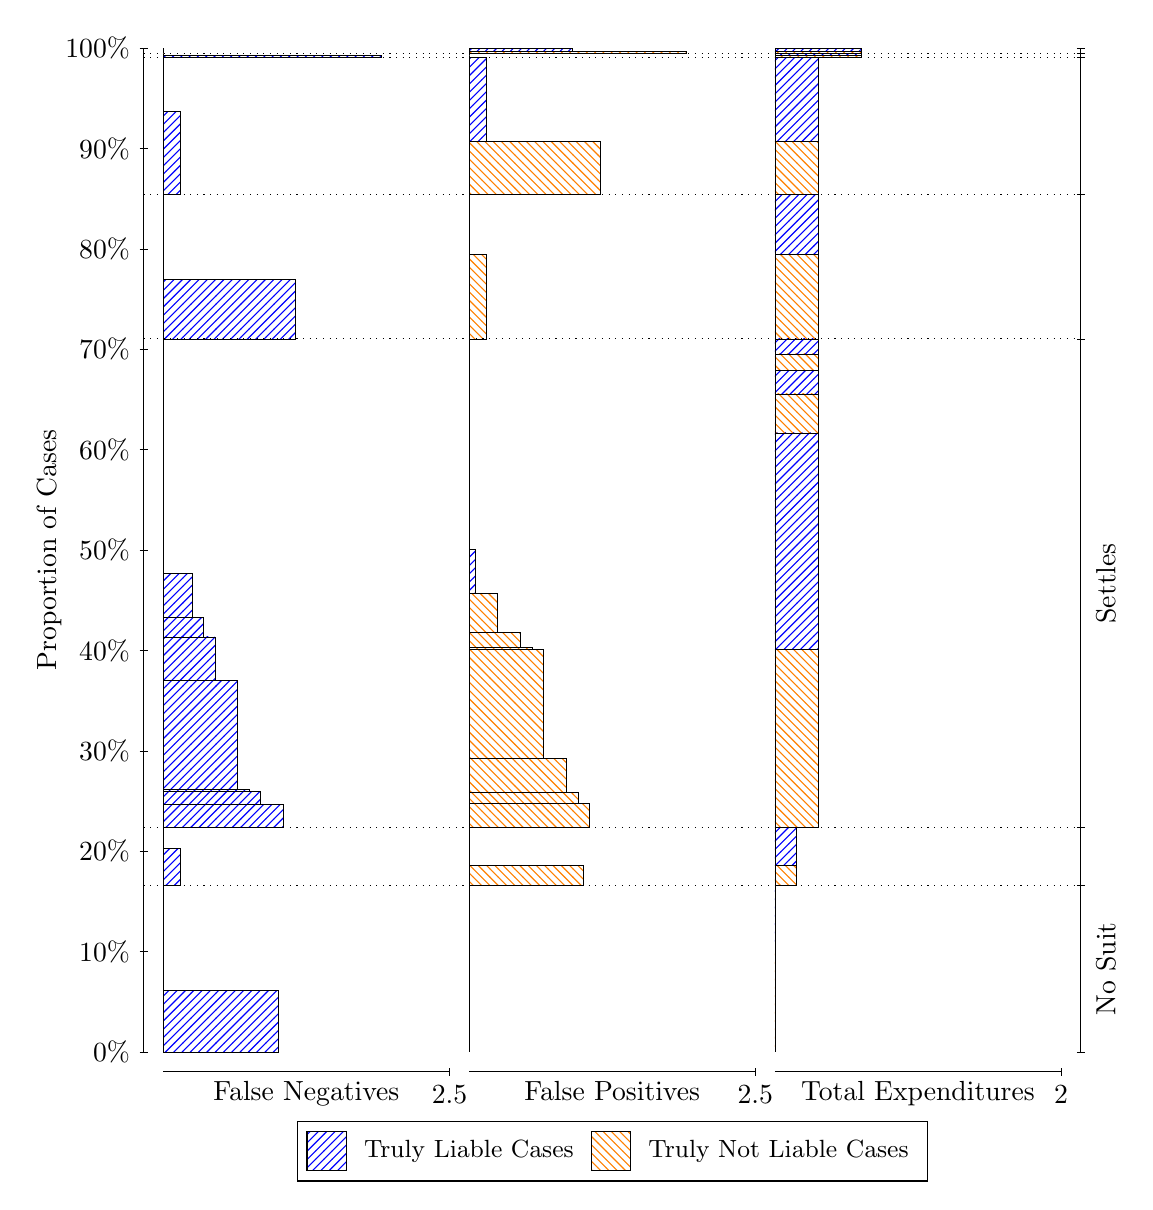
\begin{tikzpicture}
\draw[black, very thin] (1.5,1.75) -- (1.5,14.5);
\node[rotate=90, text=black, anchor=center] at (0.3, 8.125) {Proportion of Cases};
\draw[black, very thin] (1.45,1.75) -- (1.55,1.75);
\node[text=black, anchor=east] at (1.45, 1.75) {0\%};
\draw[black, very thin] (1.45,3.025) -- (1.55,3.025);
\node[text=black, anchor=east] at (1.45, 3.025) {10\%};
\draw[black, very thin] (1.45,4.3) -- (1.55,4.3);
\node[text=black, anchor=east] at (1.45, 4.3) {20\%};
\draw[black, very thin] (1.45,5.575) -- (1.55,5.575);
\node[text=black, anchor=east] at (1.45, 5.575) {30\%};
\draw[black, very thin] (1.45,6.85) -- (1.55,6.85);
\node[text=black, anchor=east] at (1.45, 6.85) {40\%};
\draw[black, very thin] (1.45,8.125) -- (1.55,8.125);
\node[text=black, anchor=east] at (1.45, 8.125) {50\%};
\draw[black, very thin] (1.45,9.4) -- (1.55,9.4);
\node[text=black, anchor=east] at (1.45, 9.4) {60\%};
\draw[black, very thin] (1.45,10.675) -- (1.55,10.675);
\node[text=black, anchor=east] at (1.45, 10.675) {70\%};
\draw[black, very thin] (1.45,11.95) -- (1.55,11.95);
\node[text=black, anchor=east] at (1.45, 11.95) {80\%};
\draw[black, very thin] (1.45,13.225) -- (1.55,13.225);
\node[text=black, anchor=east] at (1.45, 13.225) {90\%};
\draw[black, very thin] (1.45,14.5) -- (1.55,14.5);
\node[text=black, anchor=east] at (1.45, 14.5) {100\%};

\draw[black, very thin] (13.4,1.75) -- (13.4,14.5);
\draw[black, very thin] (13.35,1.75) -- (13.45,1.75);
\node[anchor=west] at (13.35, 1.75) {};
\draw[black, very thin] (13.35,3.8611) -- (13.45,3.8611);
\node[anchor=west] at (13.35, 3.8611) {};
\draw[black, very thin] (13.35,4.5974) -- (13.45,4.5974);
\node[anchor=west] at (13.35, 4.5974) {};
\draw[black, very thin] (13.35,10.806) -- (13.45,10.806);
\node[anchor=west] at (13.35, 10.806) {};
\draw[black, very thin] (13.35,12.638) -- (13.45,12.638);
\node[anchor=west] at (13.35, 12.638) {};
\draw[black, very thin] (13.35,14.378) -- (13.45,14.378);
\node[anchor=west] at (13.35, 14.378) {};
\draw[black, very thin] (13.35,14.433) -- (13.45,14.433);
\node[anchor=west] at (13.35, 14.433) {};
\draw[black, very thin] (13.35,14.5) -- (13.45,14.5);
\node[anchor=west] at (13.35, 14.5) {};

\draw[black, very thin, pattern color=blue, pattern=north east lines] (1.75,1.75) rectangle (3.2033,2.5304);
\draw[black, very thin, pattern color=orange, pattern=north west lines] (1.75,2.5304) rectangle (1.75,3.8611);
\draw[black, very thin, pattern color=blue, pattern=north east lines] (1.75,3.8611) rectangle (1.968,4.3379);
\draw[black, very thin, pattern color=orange, pattern=north west lines] (1.75,4.3379) rectangle (1.75,4.5974);
\draw[black, very thin, pattern color=blue, pattern=north east lines] (1.75,4.5974) rectangle (3.276,4.8948);
\draw[black, very thin, pattern color=blue, pattern=north east lines] (1.75,4.8948) rectangle (2.9853,5.0617);
\draw[black, very thin, pattern color=blue, pattern=north east lines] (1.75,5.0617) rectangle (2.84,5.0843);
\draw[black, very thin, pattern color=blue, pattern=north east lines] (1.75,5.0843) rectangle (2.6947,6.4715);
\draw[black, very thin, pattern color=blue, pattern=north east lines] (1.75,6.4715) rectangle (2.404,7.0209);
\draw[black, very thin, pattern color=blue, pattern=north east lines] (1.75,7.0209) rectangle (2.2587,7.2657);
\draw[black, very thin, pattern color=blue, pattern=north east lines] (1.75,7.2657) rectangle (2.1133,7.8314);
\draw[black, very thin, pattern color=orange, pattern=north west lines] (1.75,7.8314) rectangle (1.75,10.806);
\draw[black, very thin, pattern color=blue, pattern=north east lines] (1.75,10.806) rectangle (3.4213,11.565);
\draw[black, very thin, pattern color=orange, pattern=north west lines] (1.75,11.565) rectangle (1.75,12.638);
\draw[black, very thin, pattern color=blue, pattern=north east lines] (1.75,12.638) rectangle (1.968,13.7);
\draw[black, very thin, pattern color=orange, pattern=north west lines] (1.75,13.7) rectangle (1.75,14.378);
\draw[black, very thin, pattern color=blue, pattern=north east lines] (1.75,14.378) rectangle (4.5113,14.403);
\draw[black, very thin, pattern color=orange, pattern=north west lines] (1.75,14.403) rectangle (1.75,14.433);
\draw[black, very thin, pattern color=orange, pattern=north west lines] (1.75,14.433) rectangle (1.75,14.462);
\draw[black, very thin, pattern color=blue, pattern=north east lines] (1.75,14.462) rectangle (1.75,14.5);
\draw[black, very thin, pattern color=orange, pattern=north west lines] (5.6333,1.75) rectangle (5.6333,3.0807);
\draw[black, very thin, pattern color=blue, pattern=north east lines] (5.6333,3.0807) rectangle (5.6333,3.8611);
\draw[black, very thin, pattern color=orange, pattern=north west lines] (5.6333,3.8611) rectangle (7.0867,4.1206);
\draw[black, very thin, pattern color=blue, pattern=north east lines] (5.6333,4.1206) rectangle (5.6333,4.5974);
\draw[black, very thin, pattern color=orange, pattern=north west lines] (5.6333,4.5974) rectangle (7.1593,4.9094);
\draw[black, very thin, pattern color=orange, pattern=north west lines] (5.6333,4.9094) rectangle (7.014,5.0486);
\draw[black, very thin, pattern color=orange, pattern=north west lines] (5.6333,5.0486) rectangle (6.8687,5.4799);
\draw[black, very thin, pattern color=orange, pattern=north west lines] (5.6333,5.4799) rectangle (6.578,6.8659);
\draw[black, very thin, pattern color=orange, pattern=north west lines] (5.6333,6.8659) rectangle (6.4327,6.8901);
\draw[black, very thin, pattern color=orange, pattern=north west lines] (5.6333,6.8901) rectangle (6.2873,7.078);
\draw[black, very thin, pattern color=orange, pattern=north west lines] (5.6333,7.078) rectangle (5.9967,7.572);
\draw[black, very thin, pattern color=blue, pattern=north east lines] (5.6333,7.572) rectangle (5.706,8.1377);
\draw[black, very thin, pattern color=blue, pattern=north east lines] (5.6333,8.1377) rectangle (5.6333,10.806);
\draw[black, very thin, pattern color=orange, pattern=north west lines] (5.6333,10.806) rectangle (5.8513,11.879);
\draw[black, very thin, pattern color=blue, pattern=north east lines] (5.6333,11.879) rectangle (5.6333,12.638);
\draw[black, very thin, pattern color=orange, pattern=north west lines] (5.6333,12.638) rectangle (7.3047,13.316);
\draw[black, very thin, pattern color=blue, pattern=north east lines] (5.6333,13.316) rectangle (5.8513,14.378);
\draw[black, very thin, pattern color=orange, pattern=north west lines] (5.6333,14.378) rectangle (5.6333,14.408);
\draw[black, very thin, pattern color=blue, pattern=north east lines] (5.6333,14.408) rectangle (5.6333,14.433);
\draw[black, very thin, pattern color=orange, pattern=north west lines] (5.6333,14.433) rectangle (8.3947,14.462);
\draw[black, very thin, pattern color=blue, pattern=north east lines] (5.6333,14.462) rectangle (6.9413,14.5);
\draw[black, very thin, pattern color=orange, pattern=north west lines] (9.5167,1.75) rectangle (9.5167,3.0807);
\draw[black, very thin, pattern color=blue, pattern=north east lines] (9.5167,3.0807) rectangle (9.5167,3.8611);
\draw[black, very thin, pattern color=orange, pattern=north west lines] (9.5167,3.8611) rectangle (9.7892,4.1206);
\draw[black, very thin, pattern color=blue, pattern=north east lines] (9.5167,4.1206) rectangle (9.7892,4.5974);
\draw[black, very thin, pattern color=orange, pattern=north west lines] (9.5167,4.5974) rectangle (10.062,6.8659);
\draw[black, very thin, pattern color=blue, pattern=north east lines] (9.5167,6.8659) rectangle (10.062,9.613);
\draw[black, very thin, pattern color=orange, pattern=north west lines] (9.5167,9.613) rectangle (10.062,10.107);
\draw[black, very thin, pattern color=blue, pattern=north east lines] (9.5167,10.107) rectangle (10.062,10.404);
\draw[black, very thin, pattern color=orange, pattern=north west lines] (9.5167,10.404) rectangle (10.062,10.617);
\draw[black, very thin, pattern color=blue, pattern=north east lines] (9.5167,10.617) rectangle (10.062,10.806);
\draw[black, very thin, pattern color=orange, pattern=north west lines] (9.5167,10.806) rectangle (10.062,11.879);
\draw[black, very thin, pattern color=blue, pattern=north east lines] (9.5167,11.879) rectangle (10.062,12.638);
\draw[black, very thin, pattern color=orange, pattern=north west lines] (9.5167,12.638) rectangle (10.062,13.316);
\draw[black, very thin, pattern color=blue, pattern=north east lines] (9.5167,13.316) rectangle (10.062,14.378);
\draw[black, very thin, pattern color=orange, pattern=north west lines] (9.5167,14.378) rectangle (10.607,14.408);
\draw[black, very thin, pattern color=blue, pattern=north east lines] (9.5167,14.408) rectangle (10.607,14.433);
\draw[black, very thin, pattern color=orange, pattern=north west lines] (9.5167,14.433) rectangle (10.607,14.462);
\draw[black, very thin, pattern color=blue, pattern=north east lines] (9.5167,14.462) rectangle (10.607,14.5);
\draw[black, dotted] (1.5,3.8611) -- (13.4,3.8611);
\draw[black, dotted] (1.5,4.5974) -- (13.4,4.5974);
\draw[black, dotted] (1.5,10.806) -- (13.4,10.806);
\draw[black, dotted] (1.5,12.638) -- (13.4,12.638);
\draw[black, dotted] (1.5,14.378) -- (13.4,14.378);
\draw[black, dotted] (1.5,14.433) -- (13.4,14.433);
\draw[black, very thin] (1.75,1.5) -- (5.3833,1.5);
\node[text=black, anchor=north] at (3.5667, 1.5) {False Negatives};
\draw[black, very thin] (5.3833,1.45) -- (5.3833,1.55);
\node[text=black, anchor=north] at (5.3833, 1.45) {2.5};

\draw[black, very thin] (5.6333,1.5) -- (9.2667,1.5);
\node[text=black, anchor=north] at (7.45, 1.5) {False Positives};
\draw[black, very thin] (9.2667,1.45) -- (9.2667,1.55);
\node[text=black, anchor=north] at (9.2667, 1.45) {2.5};

\draw[black, very thin] (9.5167,1.5) -- (13.15,1.5);
\node[text=black, anchor=north] at (11.333, 1.5) {Total Expenditures};
\draw[black, very thin] (13.15,1.45) -- (13.15,1.55);
\node[text=black, anchor=north] at (13.15, 1.45) {2};

\node[text=black, centered, rotate=90] at (13.72, 2.8055) {No Suit};

\node[text=black, centered, rotate=90] at (13.72, 7.7017) {Settles};





\draw (7.449999999999999,1.5) node[draw=none] (baseCoordinate) {};
\begin{scope}[align=center]
        \matrix[scale=0.5, draw=black, below=0.5cm of baseCoordinate, nodes={draw}, column sep=0.1cm]{
            \node[rectangle, draw, minimum width=0.5cm, minimum height=0.5cm, pattern color=blue, pattern=north east lines] {}; &
            \node[draw=none, font=\small, text=black] (B) {Truly Liable Cases}; &
            \node[rectangle, draw, minimum width=0.5cm, minimum height=0.5cm, pattern color=orange, pattern=north west lines] {}; &
            \node[draw=none, font=\small, text=black] (B) {Truly Not Liable Cases}; \\
            };
\end{scope}

\end{tikzpicture}
\end{document}